%%%%%%%%%%%%%%%%%%%%%  kbb talk %%%%%%%%%%%%%%%%%%%%%%%%%%%%%%%
%%%%%%%%%%%%%%%%%%%%%%%%%%%%%%%%%%%%%%%%%%%%%%%%%%%%%%%%%%%%%%%

\documentclass[12pt,fleqn]{seminar}
\input{seminar.bug}
\pagestyle{empty}
\pdfhorigin=1truein
\pdfvorigin=1truein


% packages
\usepackage{ifpdf}
\usepackage{bm}
\usepackage{latexsym}
\usepackage{color}
\usepackage{pstricks}
\usepackage{ulem} %uwave
\usepackage{amsmath}

\usepackage{amssymb}
%\usepackage{float}
\usepackage{bm}
%\usepackage{wasysym}
%\usepackage[landscape]{geometry}
\usepackage{graphicx}
\usepackage{epstopdf}
\graphicspath{{./Figs/}{./}{../}}
\graphicspath{{/Users/danielhurowitz/PROJ/NEG/Figs/}{./}{../}}



% basic	commands I
\newcommand{\mass}{\mathsf{M}} 
\newcommand{\half}{\mbox{\small $\frac{1}{2}$}}
\newcommand{\sinc}{\mbox{sinc}}
\newcommand{\const}{\mbox{const}}
\newcommand{\trc}{\mbox{trace}}
\newcommand{\intt}{\int\!\!\!\!\int }
\newcommand{\ointt}{\int\!\!\!\!\int\!\!\!\!\!\circ\ }
\newcommand{\eexp}{\mbox{e}^}
\newcommand{\bra}{\left\langle}
\newcommand{\ket}{\right\rangle}
\newcommand{\EPS} {\mbox{\LARGE $\epsilon$}}
\newcommand{\ttimes} {\mbox{\tiny \ $^{\times}$ \ }}
\newcommand{\ar}{\mathsf r}
\newcommand{\im}{\mbox{Im}}
\newcommand{\re}{\mbox{Re}}
\newcommand{\bmsf}[1]{\bm{\mathsf{#1}}} 
\newcommand{\pd}[2]{\frac{\partial #1}{\partial #2}}
\newcommand{\bitem}{$\newline \ \ \bullet \ \ $} 
\newcommand{\ola}{\protect\overleftarrow}
\newcommand{\ora}{\protect\overrightarrow}

% basic	commands II
\newcommand{\hide}[1]{}
\newcommand{\tbox}[1]{\mbox{\tiny #1}}
\newcommand{\Cn}[1]{\begin{center}{#1}\end{center}}
\newcommand{\be}{\begin{eqnarray*}}
\newcommand{\ee}{\end{eqnarray*}}
\newcommand{\beq}{\begin{eqnarray*}}
\newcommand{\eeq}{\end{eqnarray*}}

\newcommand{\mpg}[2][0.45\hsize]{\begin{minipage}[b]{#1}{#2}\end{minipage}}
%
\newcommand{\bmp}[1]{\begin{minipage}[t]{#1}\noindent }
\newcommand{\smp}[1]{\end{minipage}\begin{minipage}[t]{#1}\noindent }
\newcommand{\emp}{\end{minipage}}

\newcommand{\amatrix}[1]{\begin{matrix} #1 \end{matrix}} 


% extra commands for colors
\definecolor{blk}{rgb}{0.,0.,0.}
\definecolor{red}{rgb}{1.,0.,0.}
\definecolor{green}{rgb}{0.,0.5,0.}
\definecolor{blue}{rgb}{0.,0.,1.}
\definecolor{bluek}{rgb}{0.,0.,0.5}
\definecolor{orange}{rgb}{1.,0.56.,0}
\newcommand{\cblk}[1]{\textcolor{blk}{#1}}
\newcommand{\cred}[1]{\textcolor{red}{#1}}
\newcommand{\cgreen}[1]{\textcolor{green}{#1}}
\newcommand{\cblue}[1]{\textcolor{blue}{#1}}
\newcommand{\cbluek}[1]{\textcolor{bluek}{#1}}
\newcommand{\corange}[1]{\textcolor{orange}{#1}}


% extra commands for slides

%\newcommand{\Up}[1][0.5]{\vspace{-#1cm}}
%\newcommand{\Dn}[1][0.5]{\vspace{#1cm}}
%\newcommand{\Tl}[1]{\begin{center}{\bf \small \cblue{#1}}\end{center}}

\newcommand{\Up}[1][5]{\vspace{-#1mm}}
\newcommand{\Dn}[1][5]{\vspace{#1mm}}
\newcommand{\Tl}[1]{\begin{center}{\bf \small \cblue{#1}}\end{center}}

\renewcommand{\slideparindent}{0mm}
\setlength{\mathindent}{0cm} 

% \newcommand{\newsld}{\end{slide}\begin{slide}}


\newcommand{\bslA}[1]{
%portrait
\pdfpagewidth=210truemm
\pdfpageheight=297truemm
\pdfhorigin=1truein
\pdfvorigin=1truein
%portrait
\renewcommand{\slidetopmargin}{0mm}
\renewcommand{\slideleftmargin}{-54mm}
\setlength{\slidewidth}{190mm}
\setlength{\slideheight}{277mm}
\begin{slide}
}



\newcommand{\bslB}[1]{
%landscape
\pdfpagewidth=297truemm
\pdfpageheight=210truemm
\pdfhorigin=1truein
\pdfvorigin=1truein
%portrait 
\renewcommand{\slidetopmargin}{0mm}
\renewcommand{\slideleftmargin}{33mm}
\setlength{\slideheight}{190mm}
\setlength{\slidewidth}{150mm} %130
%portrait fonts
\begin{slide}
\ptsize{8}
}



\newcommand{\bslC}[1]{
%landscape
\pdfpagewidth=297truemm
\pdfpageheight=210truemm
\pdfhorigin=1truein
\pdfvorigin=1truein
%landscape
\renewcommand{\slidetopmargin}{0mm}
\renewcommand{\slideleftmargin}{33mm}
\setlength{\slideheight}{190mm}
\setlength{\slidewidth}{277mm}
%portrait fonts
\begin{slide}
\ptsize{8}
}



\newcommand{\bslD}[1]{
%landscape
\pdfpagewidth=297truemm
\pdfpageheight=210truemm
\pdfhorigin=1truein
\pdfvorigin=1truein
%landscape
\renewcommand{\slidetopmargin}{0mm}
\renewcommand{\slideleftmargin}{33mm}
\setlength{\slideheight}{190mm}
\setlength{\slidewidth}{277mm}
%landscape fonts
\begin{slide}
}



\newcommand{\esl}{\end{slide}}


\newcommand{\vbar}{
\begin{picture}(1,1)
\thicklines
\put(0,61){ \ \ \line(0,-1){280} \ \ } 
\end{picture} 
}


%%%%%%%%%%%%%%%%%%%%%%%%%%%%%%%%%%%%%%%%%%%%%%%%%%%%%%%%%%%%%%%%%%%
%%%%%%%%%%%%%%%%%%%%%%%%%%%%%%%%%%%%%%%%%%%%%%%%%%%%%%%%%%%%%%%%%%%


%%%%%%%%%%%%%%%%%%%%%%%%%%%%%%%%%%%%%%%%%%%%%%%%%%%%%%%%%%%%%%%%%%%
%%%%%%%%%%%%%%%%%%%%%%%%%%%%%%%%%%%%%%%%%%%%%%%%%%%%%%%%%%%%%%%%%%%
\begin{document}
%%%%%%%%%%%%%%%%%%%%%%%%%%%%%%%%
\bslD

\Tl{\Large{Percolation, sliding, localization and relaxation in glassy circuits }}


\Cn{\bf Daniel Hurowitz, Doron Cohen,\\ \corange{Ben-Gurion University}}
%
%
%\bmp{0.5\hsize}
%
%
%
%%\Cn{ \includegraphics[ height=4cm]{}}
%
%\smp{0.5\hsize}
%
%\vspace{0.2cm}
%
%
%
%%{\includegraphics[height=3cm]{ResistorsNetworkBath_a}}
%
%\emp
%
%\bmp{\hsize}



\bmp{0.5\hsize}

\Cn{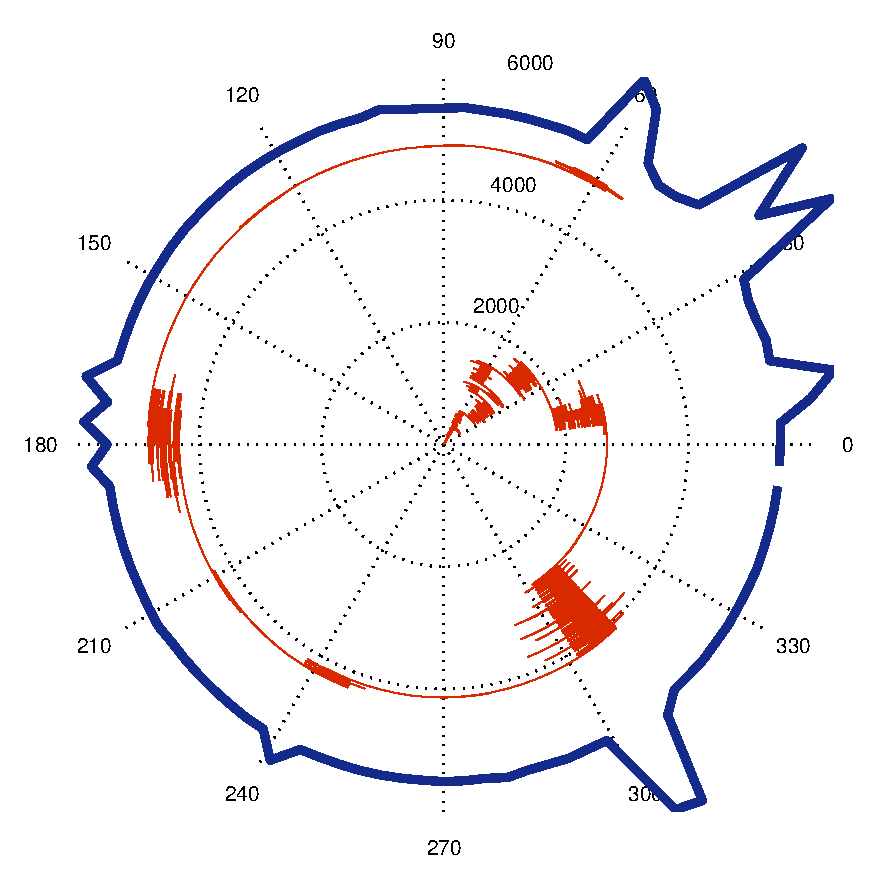
\includegraphics[height=5cm]{/Figs/polar_1_a.eps}}

\smp{0.5\hsize}

\Cn{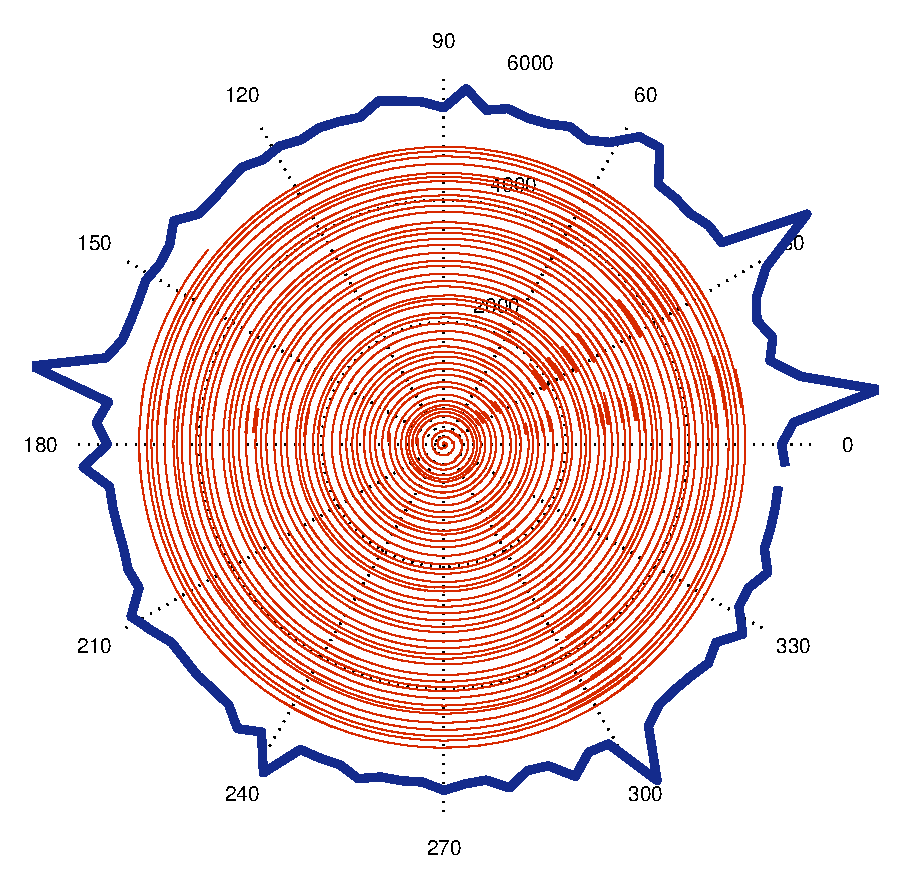
\includegraphics[height=5cm]{/Figs/polar_2_a.eps}}

\emp

\center{{   D. Hurowitz and D. Cohen, \texttt{arXiv} (2014)}}


%\emp

\esl


%%%%%%%%%%%%%%%%%%%%%%%%%%%%%%%%
\bslC

\Tl{\large Brownian motion}


\bmp{0.6\hsize}

\cgreen{{\bf Simple random walk} [Einstein]} \\
uniform lattice - all rates are equal

\smp{0.4\hsize}



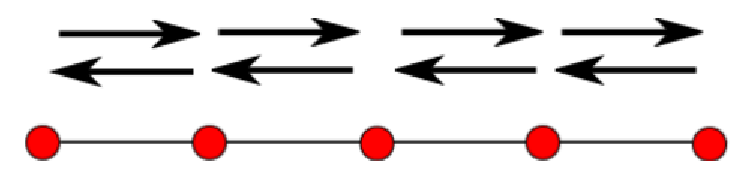
\includegraphics[width=4.5cm]{rw1a}

\emp

\bmp{0.6\hsize}

\cgreen{{\bf Random walk on disordered lattice} [Alexander et. al]} 
random lattice - random, symmetric rates

\smp{0.4\hsize}

\emp

\bmp{0.6\hsize}

\cgreen{{\bf Random walk in random environment} [Sinai, Derrida]} 

rates allowed to be asymmetric

\smp{0.4\hsize}

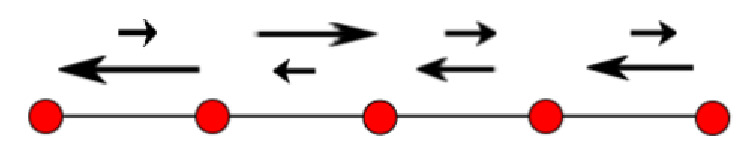
\includegraphics[width=4.5cm]{rw2a}

\emp



Dynamics described conservative rate equation


\beq
\frac{d\bm{p}}{dt} \ \ = \ \ \bm{W} \bm{p},  \ \ \ \ \ 
\bm{W} \ \ = \ \ \left[\amatrix{
-\gamma_1   & w_{1,2}   & 0         & ... \\ 
w_{2,1}     & -\gamma_2 & w_{2,3}   & ... \\ 
0           & w_{3,2}   & -\gamma_3 & ... \\
...         & ...       & ...       & ...
}\right], \ \ \ \ \ \sum_n w_{nm} = 0
\eeq

{transition rates across } $n^{th}$ bond $w_n\eexp{\pm\mathcal{E}_n/2}$

\bmp{0.5\hsize}


{Stochastic field} \ \ $\displaystyle \mathcal{E}_n  \sim  [s-\sigma, s+\sigma]$

{Affinity / Bias}\ \  $\displaystyle s = \frac{1}{N} \sum \mathcal{E}_n \equiv \frac{\mathcal{S}_{\circlearrowleft}}{N} $

{Resistor network} $\displaystyle P(w) \propto w^{\alpha-1}$


\smp{0.5\hsize}

How do spectral properties of ${\bm W}$ depend on 

\Cn{$(\alpha,\sigma, s)$?}

\emp
%
\esl


\bslC

\Tl{\large{Sinai spreading}}

\bmp{0.55\hsize}

\Up

\be
\cgreen{\text{Stochastic field:}} \ \ 
\mathcal{E}_n \ \equiv \ \ln \left[\frac{{w}_{n+1,n}}{{w_{n,n+1}}}\right]  \ ,  
\hspace{1cm} \cred{\sigma = \sqrt{\mbox{Var} (\mathcal{S}_n)}}
\ee


\be
\text{\cgreen{Stochastic Motive Force:} } \ \ 
\mathcal{S}_{\circlearrowleft} = 
\sum_{n\in\text{ring}} \ \ln \left[ \ \frac{\ora{w}_n}{\ola{w}_n} \ \right ] 
\ee

\be
\text{\cgreen{If}} \ \ \ \frac{\ora{w}_n}{\ola{w}_n}=\exp\left[-\frac{E_n-E_{n-1}}{T} \right] 
\ \ \ \cgreen{\leadsto} \ \ \  
\mathcal{S}_{\circlearrowleft}  \ = \ 0
\ee


\be
\text{\cgreen{Affinity}}: \ \ s \  = \ \frac{\mathcal{S}_{\circlearrowleft}}{N}
\ee


\Dn


\cgreen{For small $s$} [1]:

Sub-diffusive spreading $x \ \sim \ [\log (t)]^2$,

Exponentially small drift $\displaystyle v  \ \sim \ e^{-\sqrt{N}}$.
 

\Dn

\cgreen{For arbitrary $s$} [2,3]: 

Complicated expressions for $v$ and $D$.

{\bf sliding transition}

\Dn



\smp{0.45\hsize}

\hspace*{1cm}
\includegraphics[height=25mm]{sparse_network2.eps}

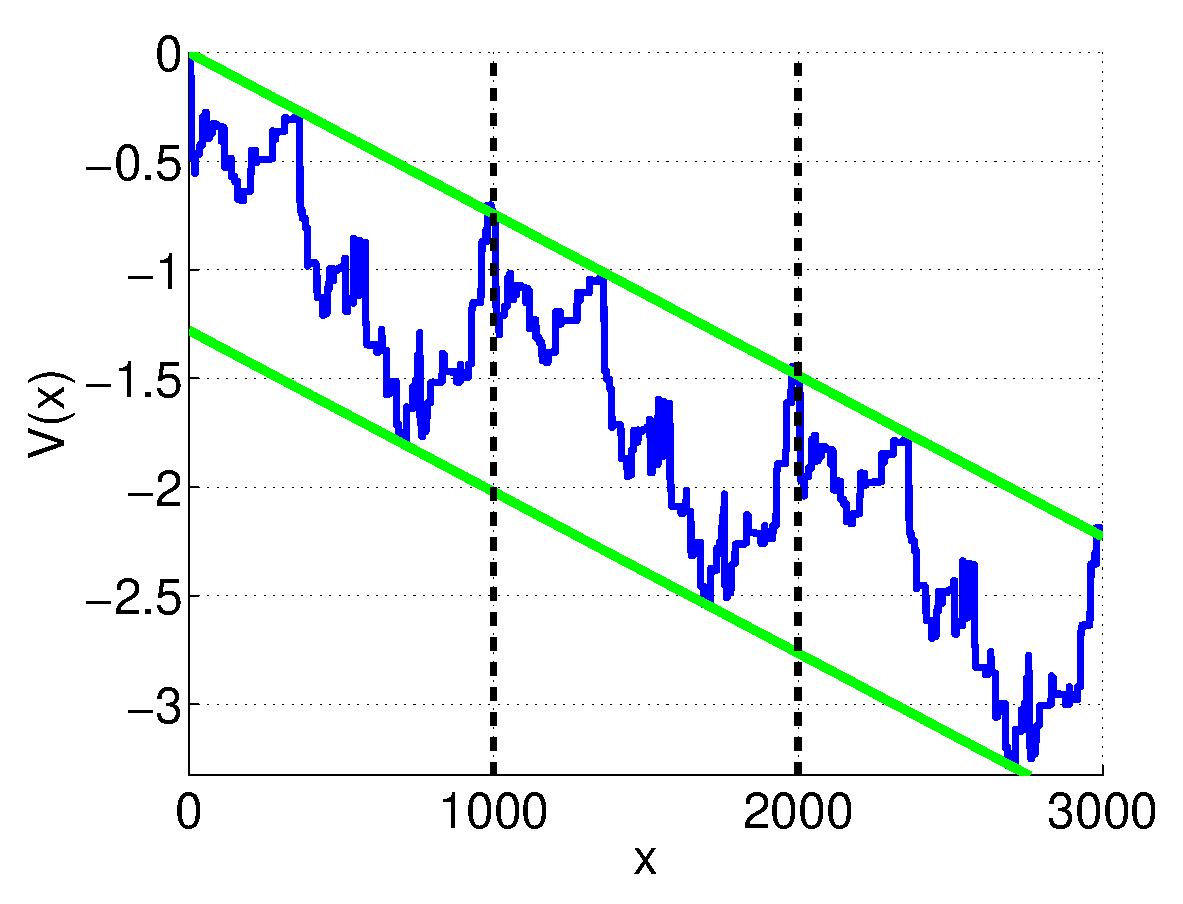
\includegraphics[height=3.5cm]{V_x}

\Dn[2]

[1] {\bf Sinai} (1982)

[2] {\bf Derrida} (1983)

[3] {\bf Aslangul, Pottier, Saint-James}  (1989)

\Dn[2]

\cred{\bf ESR is violated for large $s$}

\emp


\esl

%%%%%%%%%%%%%%%%%%%%%%%%%%%%%%%%%%%%%%%%%%
\bslC

\Tl{The spectrum}

\bmp{0.5\hsize}

\Cn{
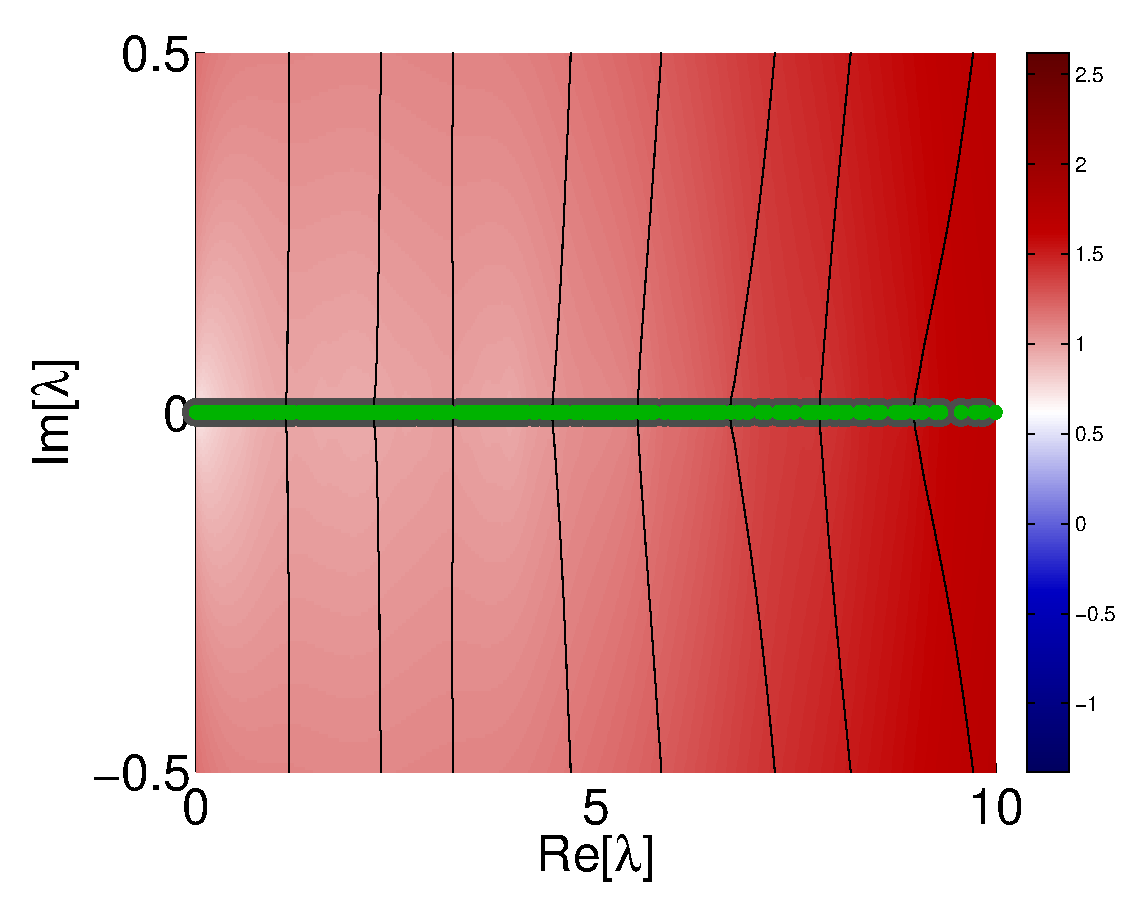
\includegraphics[height=3.5cm]{spectrum_electrostatics1_2}
}
\smp{0.5\hsize}

\Cn{
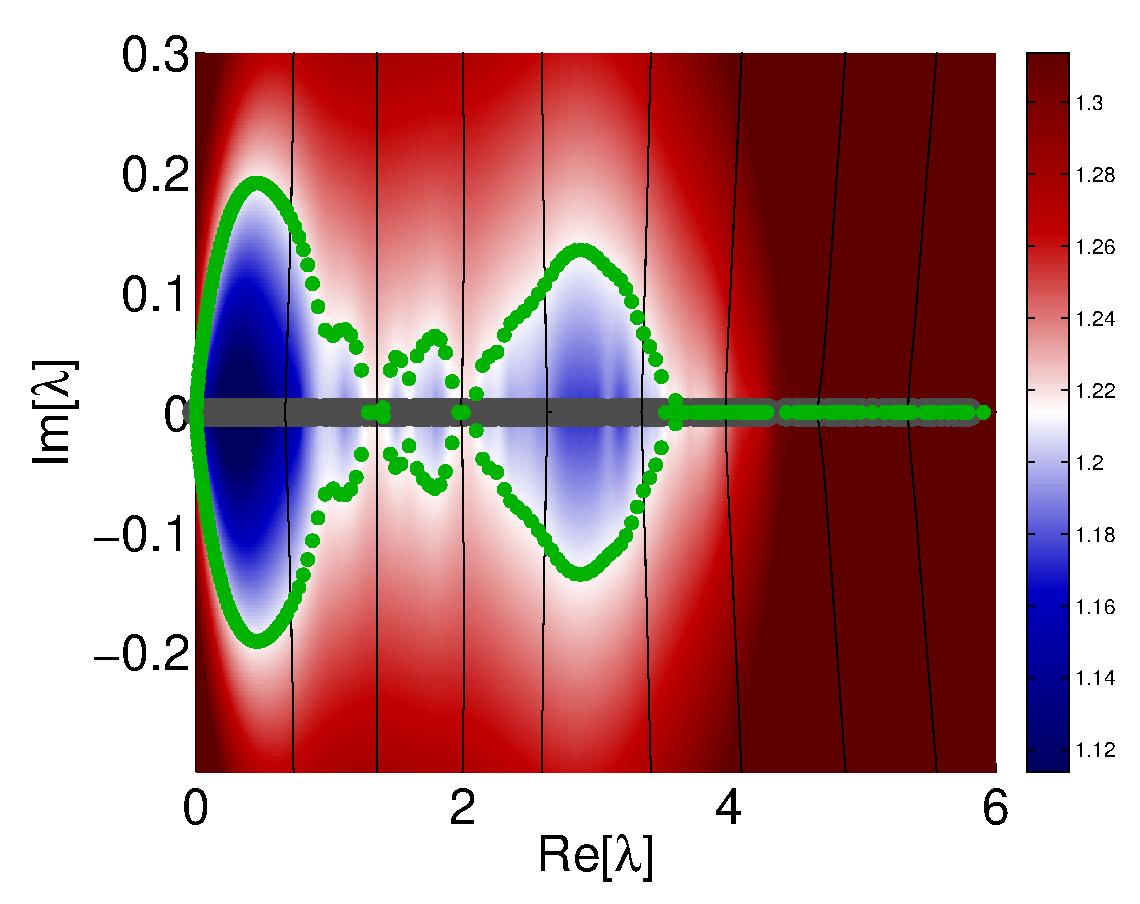
\includegraphics[height=3.5cm]{spectrum_electrostatics1}
}

\emp 

\bmp{0.5\hsize}

\Cn{
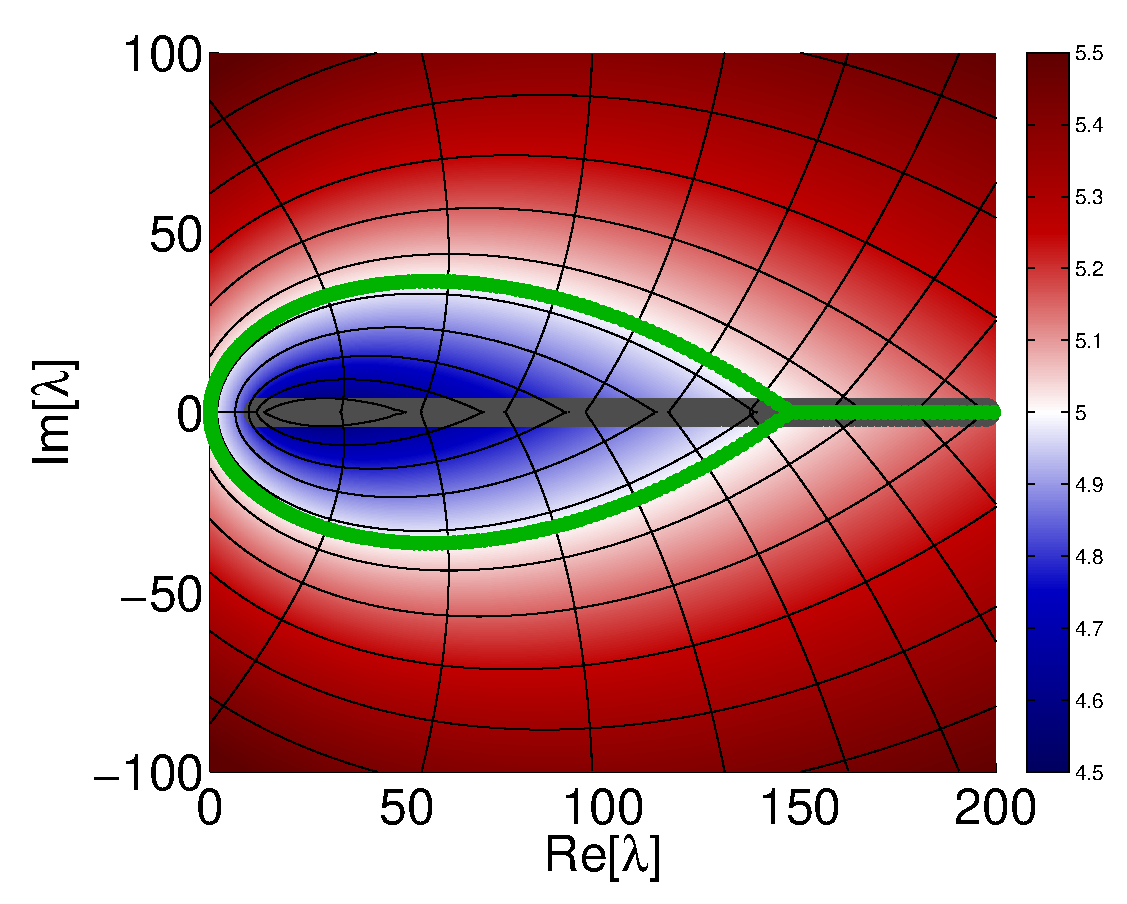
\includegraphics[height=3.5cm]{spectrum_electrostatics2}
}

\smp{0.5\hsize}

\Cn{
\includegraphics[height=3.5cm]{numComplex_100_alpha_sigma}
}

\emp

\Cn{

\cred{\bf What is the threshold bias $s_c$ for complex eigenvalues (delocalization)?}

\cred{\bf How is $s_c$ related to the percolation transition? to the sliding transition?}
}


\esl
%%%%%%%%%%%%%%%%%%%%%%%%%%%%%%%%%%%%%%%%%%%%%%%%%



%%%%%%%%%%%%%%%%%%%%%%%%%%%%%%%%%%%%%%%%%%

\bslC

\Tl{The spectral equation}

Gauge away disorder
$
{\tilde{\bm{W}} = \eexp{{\bm{U}/2}} \bm{W} \eexp{-{\bm{U}/2}}}
$
%

Associated hermitian matrix ${\bm H}$ with real eigenvalues $\epsilon_k(s)$ by setting $\mathcal{S}_{\circlearrowleft} =0$

Spectral determinant for complex eigenvalues $z$
%
\beq
\prod_{k=1}^N \left(\frac{z+\epsilon_k(s)}{\overline{w}}\right) \ \ = \ \ 2\left[\cosh\left(\frac{S_{\circlearrowleft}}{2}\right)-1\right]
\eeq
%

\Tl{Electrostatic pitcture}

\beq
\Psi(z) \ \ = \ \ \sum_k \ln\left(z-\epsilon_k\right) \ \ \equiv \ \ V(x,y)+iA(x,y)
\eeq


\esl
%%%%%%%%%%%%%%%%%%%%%%%%%%%%%%%%%%%%%%%%%%

\end{document}


